\subsection{Data Set}
The portrait data set is used for the image stylization, which segment the portrait in the selfie for the style conversion. It is a simple single-target portrait segmentation problem that is applied in the segmentation of complex scenes.
\begin{figure}[ht]
    \centering
    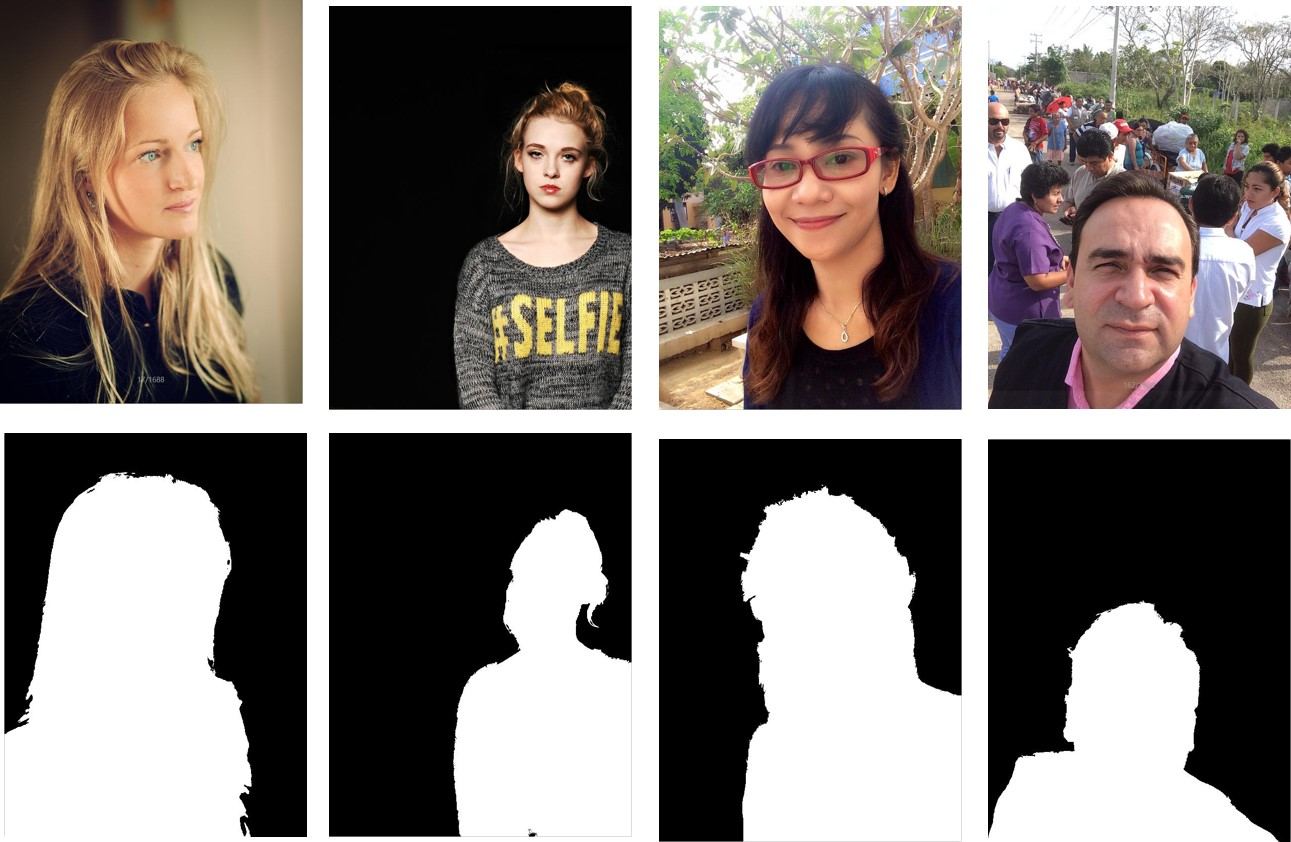
\includegraphics[width = 7cm]{figs/PortraitDataSet.jpg}
    \caption{Some images and ground truth of the Portrait data set.}\label{fig: Some images and ground truth of Portrait data set}
\end{figure}
Some images and ground truth of the portrait data set are shown in Fig. \ref{fig: Some images and ground truth of Portrait data set}. There are $1800$ portrait images in total, each of which is automatically scaled and cropped to $600\times800$, so every image is a standard portrait. The $1800$ labeled images data set are split into a $1500$ image training data set and a $300$ image testing data set by Shen et al. \cite{FCN:segmentation:shen2016automatic}. Because the images in the Portrait data set is labeled with the \emph{Photoshop} quick selection, there is some noise in ground truth as shown in Fig. \ref{fig: Some noise in the Portrait data set}.
\begin{figure}[h]
    \centering
    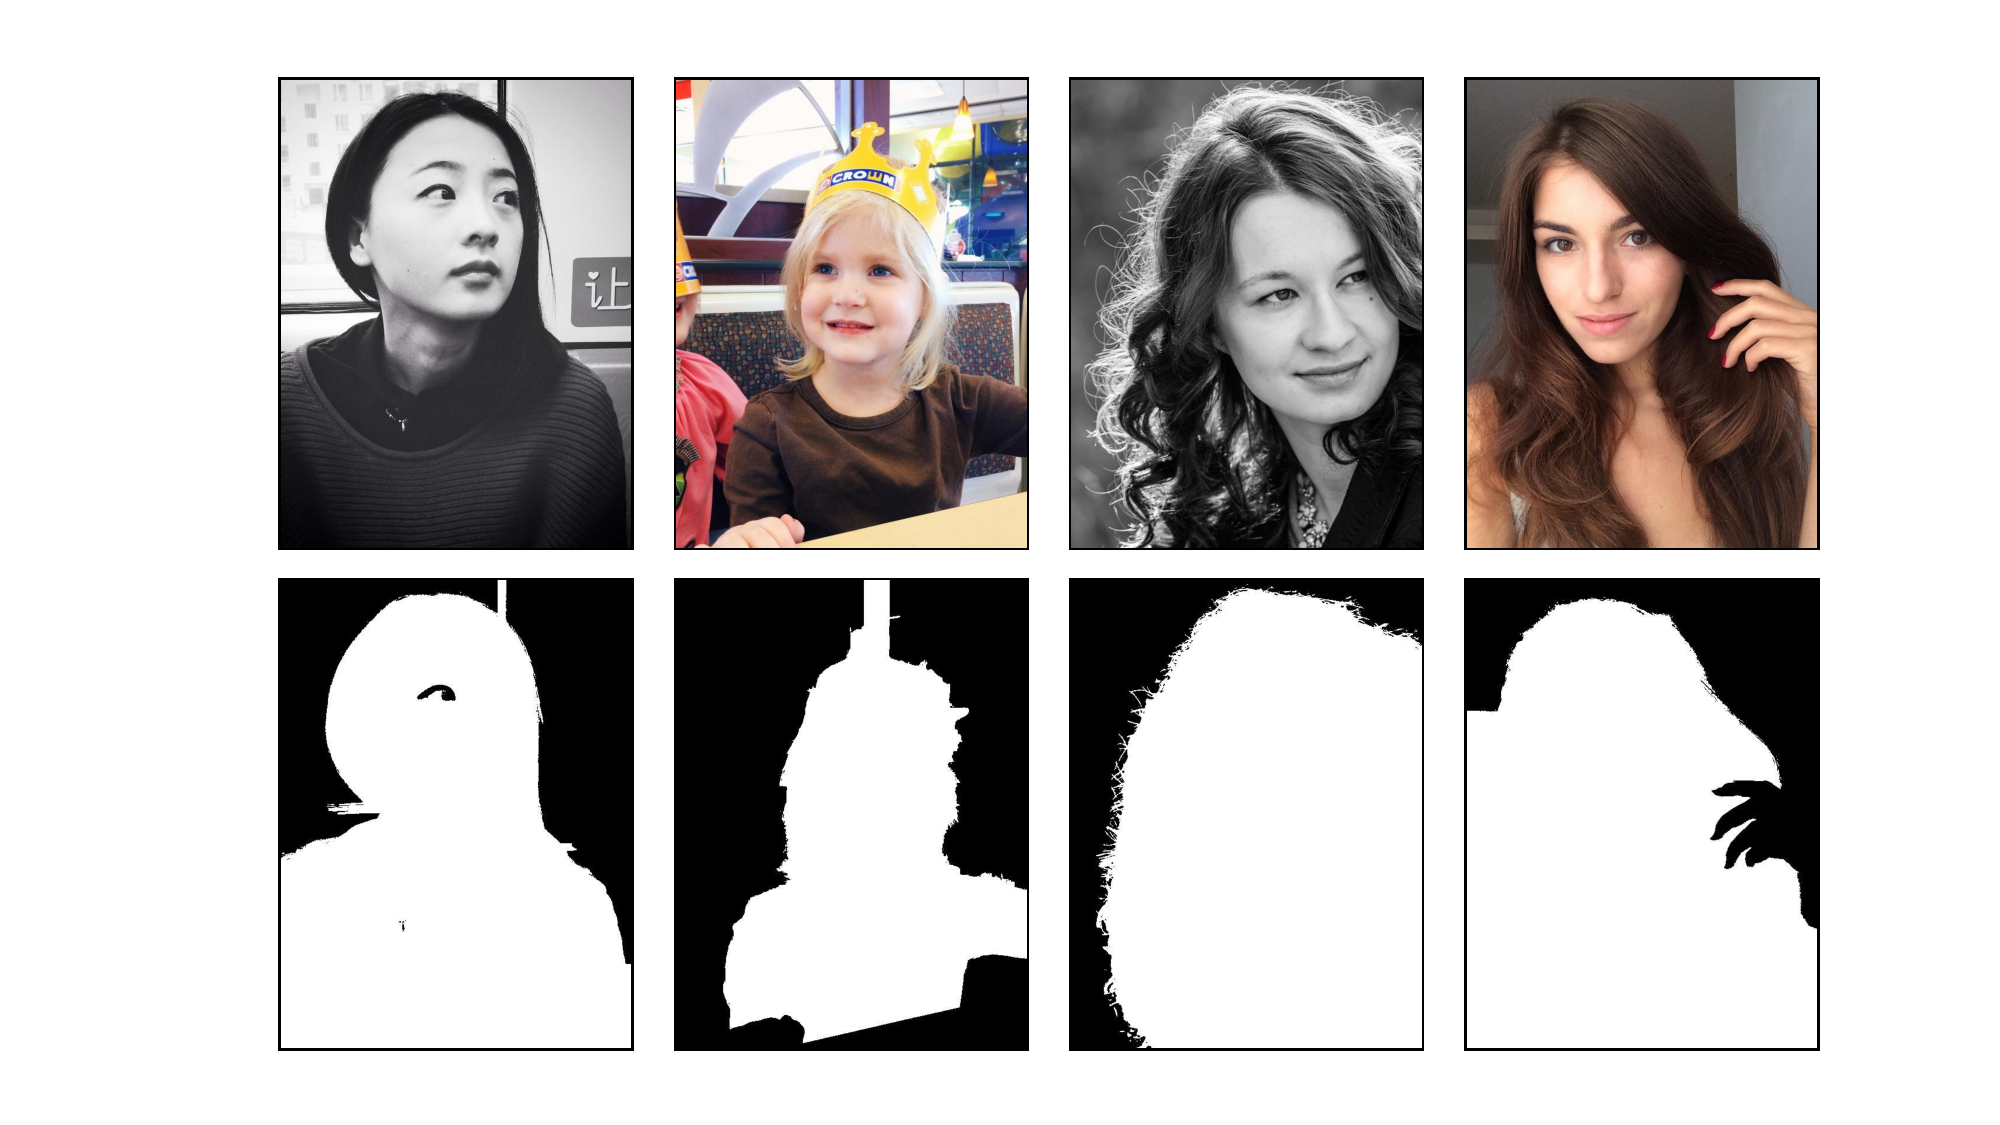
\includegraphics[width = 7cm]{figs/DataSetNoisy.eps}
    \caption{Some noise in the Portrait data set.}\label{fig: Some noise in the Portrait data set}
\end{figure}

\subsection{Evaluation Measure}
There is only one kind of the segmentation target in this image segmentation task, and only the regions of the target need to be marked. So we only need to calculate the difference between the output regions of models and the regions of ground truth. The standard metric Interaction-over-Union (IoU) is selected to represent the segmentation error.
\begin{equation}\label{eq: IOU}
    \text{IoU} = \frac{\text{Area}(\text{Output} \cap \text{Ground Truth})}{\text{Area}(\text{Output} \cup \text{Ground Truth})}
\end{equation}
Eq. (\ref{eq: IOU}) is calculated by dividing the intersection area and the union area of the region of output and ground truth. Finally, the mean IoU of $300$ testing images is used to verify the performance of different models.

\subsection{Implementation}
All FCNs are trained with Caffe \cite{FCN:caffe:jia2014caffe}, and all parameters are given by Shen et al. \cite{FCN:segmentation:shen2016automatic}. The probability map is obtained from PortraitFCN and PortraitFCNplus, which are trained with the Portrait data set.
It can be seen from Fig. \ref{fig: Some results of the GAT} that it is already very close to the shape of the probability map at the second iteration, so the number of GAT iterations is set to $2$. The level set function $\phi$ is initialized with the probability map, and extended to intervals $[-200, 200]$. The same parameters are used in all testing images, and the parameters are listed int Table \ref{table: Parameters of the proposed method}.
\begin{table}[h]
    \centering
    \caption{Parameters of the proposed method.}\label{table: Parameters of the proposed method}
    \begin{tabular}{c|c|c}
        \hline
        \hline
        Parameter & Value & Reference \\
        \hline
        $\epsilon$ & 0.5 & Eq. (\ref{eq: equation epsilon}) \\
        $\sigma$ & 4 & Eq. (\ref{eq: gaussian sigma}) \\
        $\lambda_1$ & 20 & Eq. (\ref{eq: Level Set 1-item}) \\
        $\lambda_2$ & 20 & Eq. (\ref{eq: Level Set 1-item}) \\
        $\pi_1$ & 2*500 & Eq. (\ref{eq: Level Set 2-item}) \\
        $\pi_2$ & 2*500 & Eq. (\ref{eq: Level Set 2-item}) \\
        $\nu$ & 0.5*255*255 & Eq. (\ref{eq: Level Set 3-item}) \\
        $\mu$ & 1.0 & Eq. (\ref{eq: Level Set 4-item}) \\
        $\Delta t$ & 0.2 & Eq. (\ref{eq: iter Level Set}) \\
        \hline
        \hline
    \end{tabular}
\end{table}
% \footnote{The codes are available at https://github.com/zsh965866221/LevelSet-ShapePrior-DeepLearning}

\subsection{Result and Analysis}\label{subsec: Result and Analysis}
In this paper, we mainly compare with PortraitFCN and PortraitFCNplus \cite{FCN:segmentation:shen2016automatic}, which is equivalent to an attempt at the image segmentation task with combining of the level set method and FCNs. FCN8s is a CNN structure proposed by Long et al. \cite{FCN-original:long2015fully}, and trained with the Pascal VOC data set \cite{FCN:DataSet:Everingham15}. There are $21$ different classes in the Pascal VOC data set, but the Portrait data set used in this paper has $1$ class, so only the person class in FCN8s is used. The PortraitFCN is the retrain of FCN8s at Portrait data set. The PortraitFCNplus expands the $3$-channel of the original image into $6$-channel based on the PortraitFCN, adding the mean mask and normalized x and y. The mean mask is shown in Fig. \ref{fig: The standard shape mask}. In this paper, the output of PortraitFCN and PortraitFCNplus are selected as the probability maps respectively to verify the performance of the proposed method.

Finally, the performance comparison of different models at Portrait data set is shown in Table \ref{table: Performance comparson of different models}, and the contour evolution process of proposed level set method with PortraitFCN at Portrait data set is shown in Fig. \ref{fig: The contour evolution process of proposed Level Set method at Portrait data set}. The picture below in Fig. \ref{fig: The contour evolution process of proposed Level Set method at Portrait data set} is the evolution process. The blue curve is the contour by the probability map with PortraitFCN, and the red one is the proposed level set method.
\begin{table}[h]
    \centering
    \caption{Performance comparison of different models at Portrait data set.}\label{table: Performance comparson of different models}
    \begin{tabular}{c|c}
        \hline
        \hline
        \textbf{Methods} & \textbf{Mean IoU} \\
        \hline
        FCN(Person Class) & 73.09\% \\
        PortraitFCN & 94.20\% \\
        PortraitFCN + Proposed & 95.17\% \\
        PortraitFCNplus & 95.91\% \\
        PortraitFCNplus + Proposed & 95.74\% \\
        \hline
        \hline
    \end{tabular}
\end{table}
\begin{figure}[ht]
    \centering
    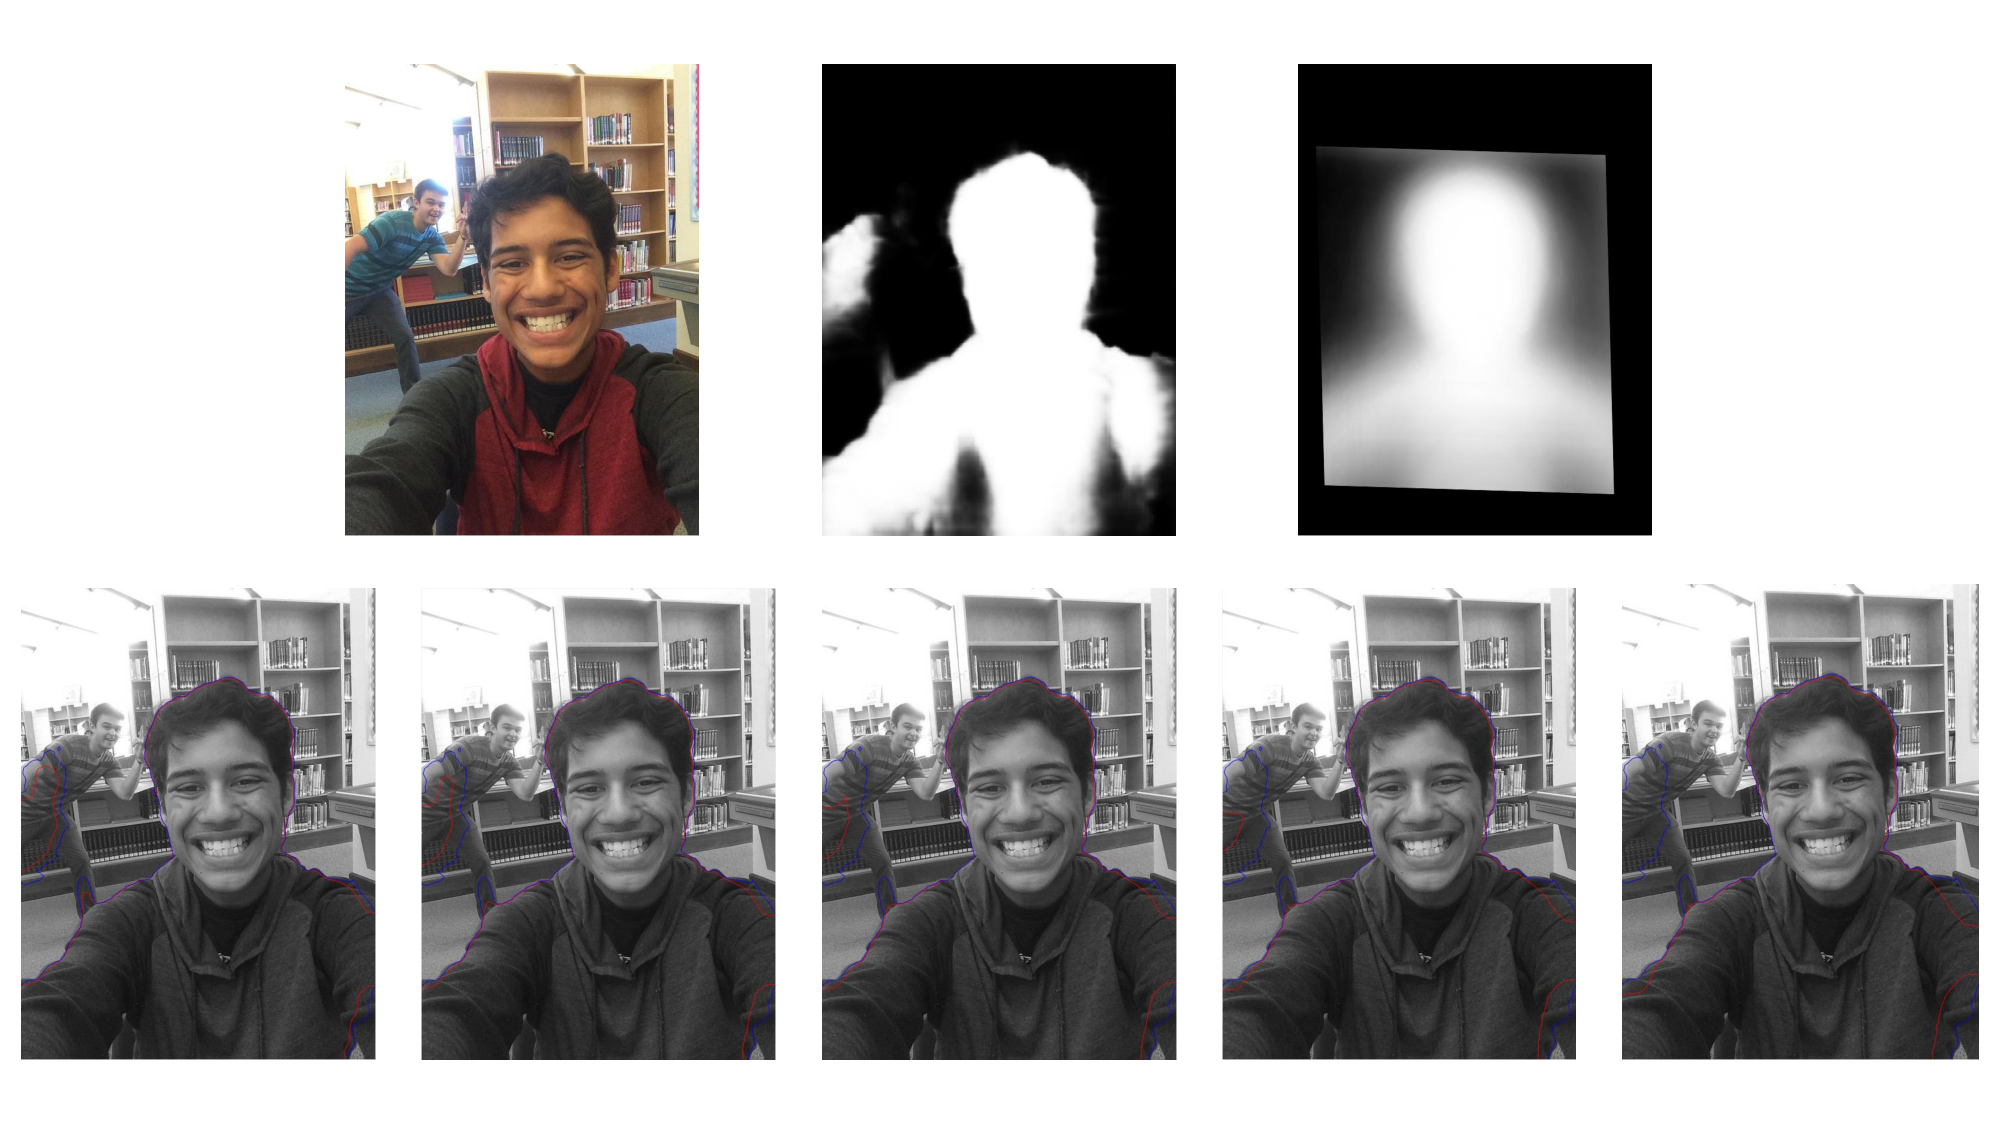
\includegraphics[width=8.8cm]{figs/LevelSet_Result.eps}
    \caption{The contour evolution process of proposed method at Portrait data set.}
    \label{fig: The contour evolution process of proposed Level Set method at Portrait data set}
\end{figure}

It can be seen from Table \ref{table: Performance comparson of different models} that the proposed method gets great improvement with PortraitFCN, but some weakening with PortraitFCNplus. As shown in Fig. \ref{fig: Some results of the GAT}, the output of PortraitFCN have some shortcomings of noisy, non-smooth, imprecise at boundary and no shape prior in Subsection \ref{subsec: FCNs for the Probability Map}. The proposed method solves the problem of the shape prior, so it is effective with PortraitFCN. However, with PortraitFCNplus, the mean mask has been added in the training process and achieved a great performance at most of the pictures. Because of the imprecise of the corrected shape prior, the original probability map information would be disturbed during the evolution of the level set, which degrades the performance. It can be seen from Fig. \ref{fig: The contour evolution process of proposed Level Set method at Portrait data set} that the regions far from the corrected prior shape would be erased during the iterative process. But the region in the lower right corner of the image is considered to have a low probability, so it is also erased.

\subsection{The Results of Different Reference Information}
In this subsection, a series of experiments are conducted to verify the availability of different reference information on the segmentation result. An image form the Portrait data set is used to analyze the result. And the image, the probability map from PortraitFCN and the corrected shape prior are shown in Fig. \ref{fig: The image, the probability map and the corrected shape prior for experiments}.
\begin{figure}[h]
    \centering
    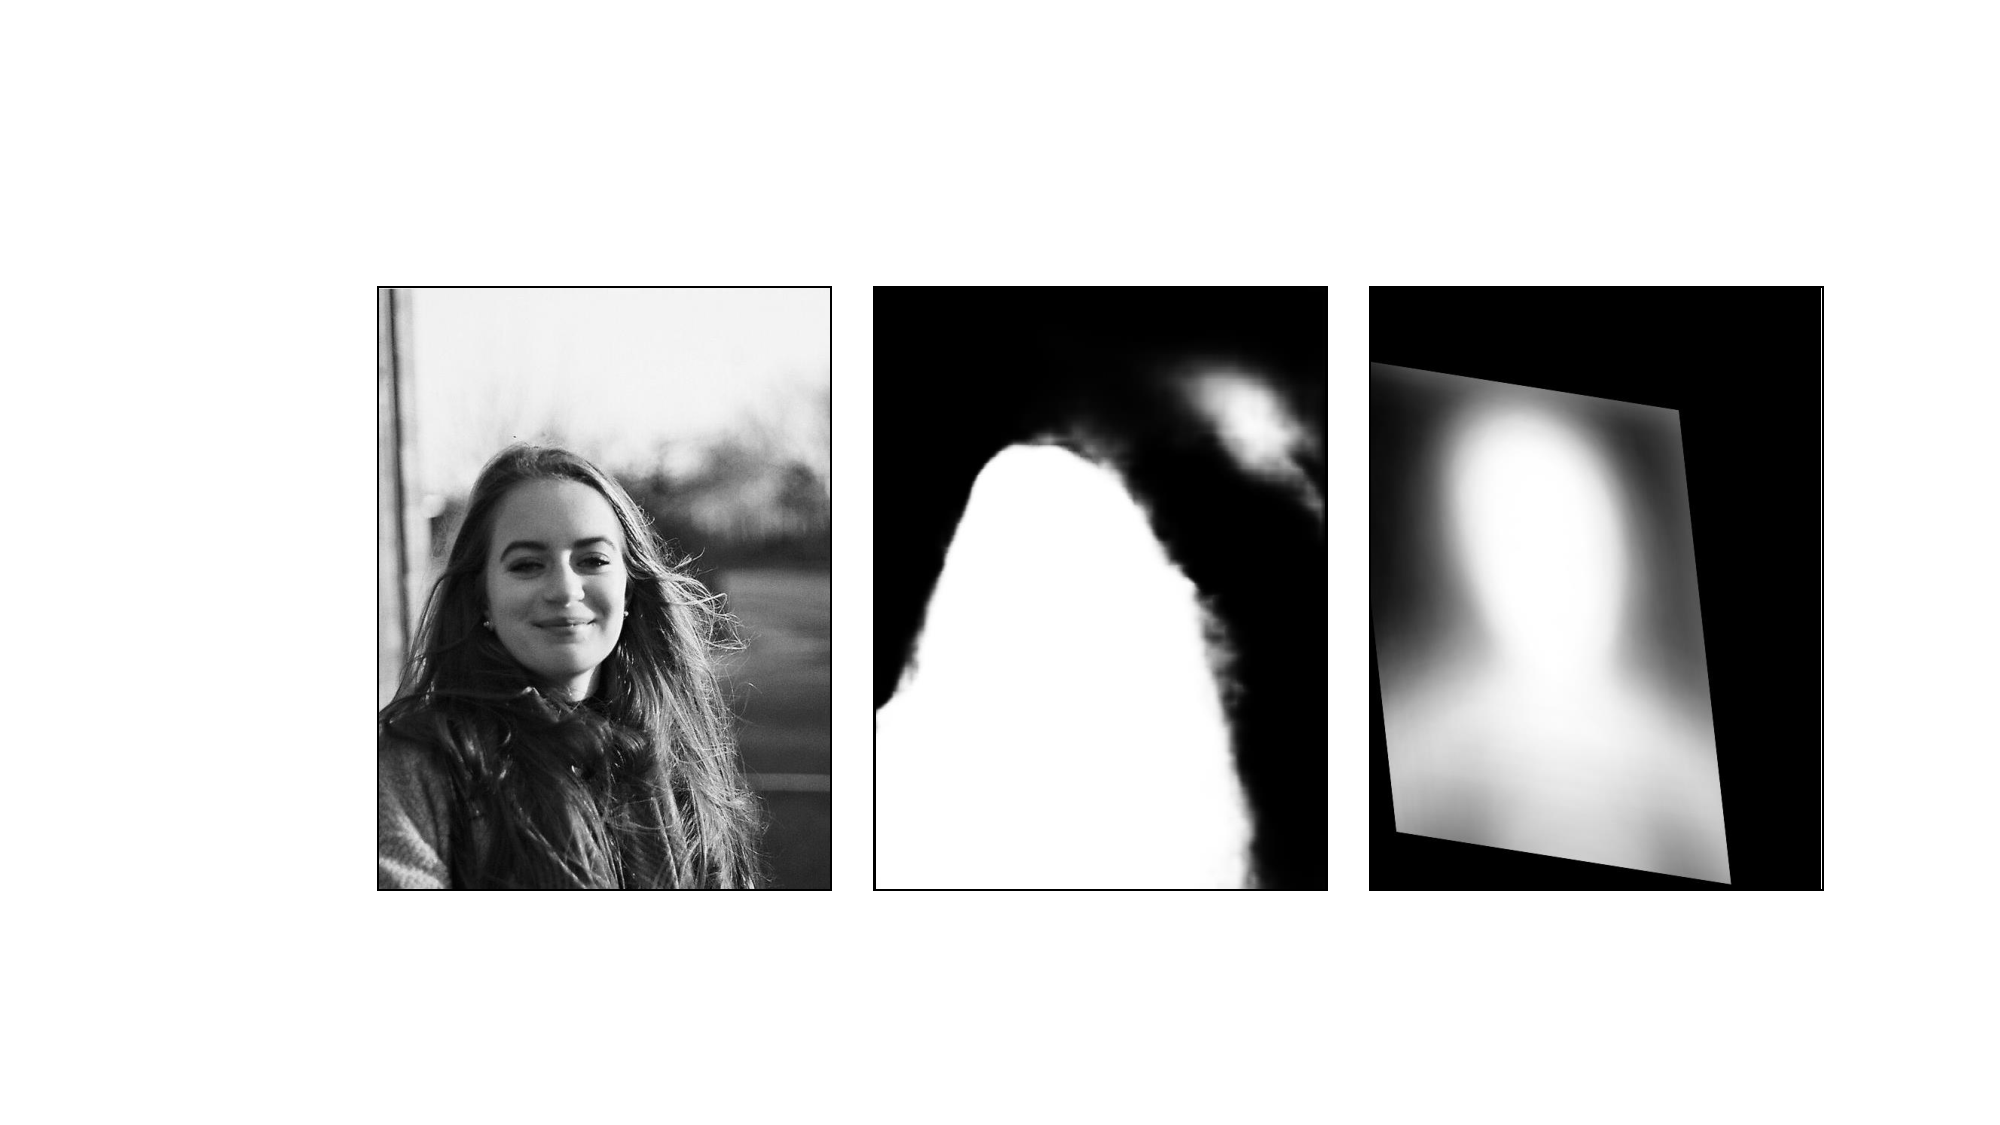
\includegraphics[width=7cm]{figs/DifferentInformation_image.eps}
    \caption{The image, the probability map and the corrected shape prior for experiments.}
    \label{fig: The image, the probability map and the corrected shape prior for experiments}
\end{figure}

\subsubsection{Experiment $1$}
The reference information selected in Experiment $1$ uses the original image and the probability map information in $\mathcal{E}_{\text{img}}$ like Subsection \ref{subsec: Level Set Method for Image Segmentation}, so that the regions that are close to each other in pixels and satisfy the probability map are grouped together. And $\mathcal{E}_{\text{shape}}$ just uses the corrected prior shape, which ensures the similarity of the final segmentation and the corrected shape prior. The contour evolution process of Experiment $1$ is shown in Fig. \ref{fig: The contour evolution process of Experiment 1}.
\begin{figure}[ht]
    \centering
    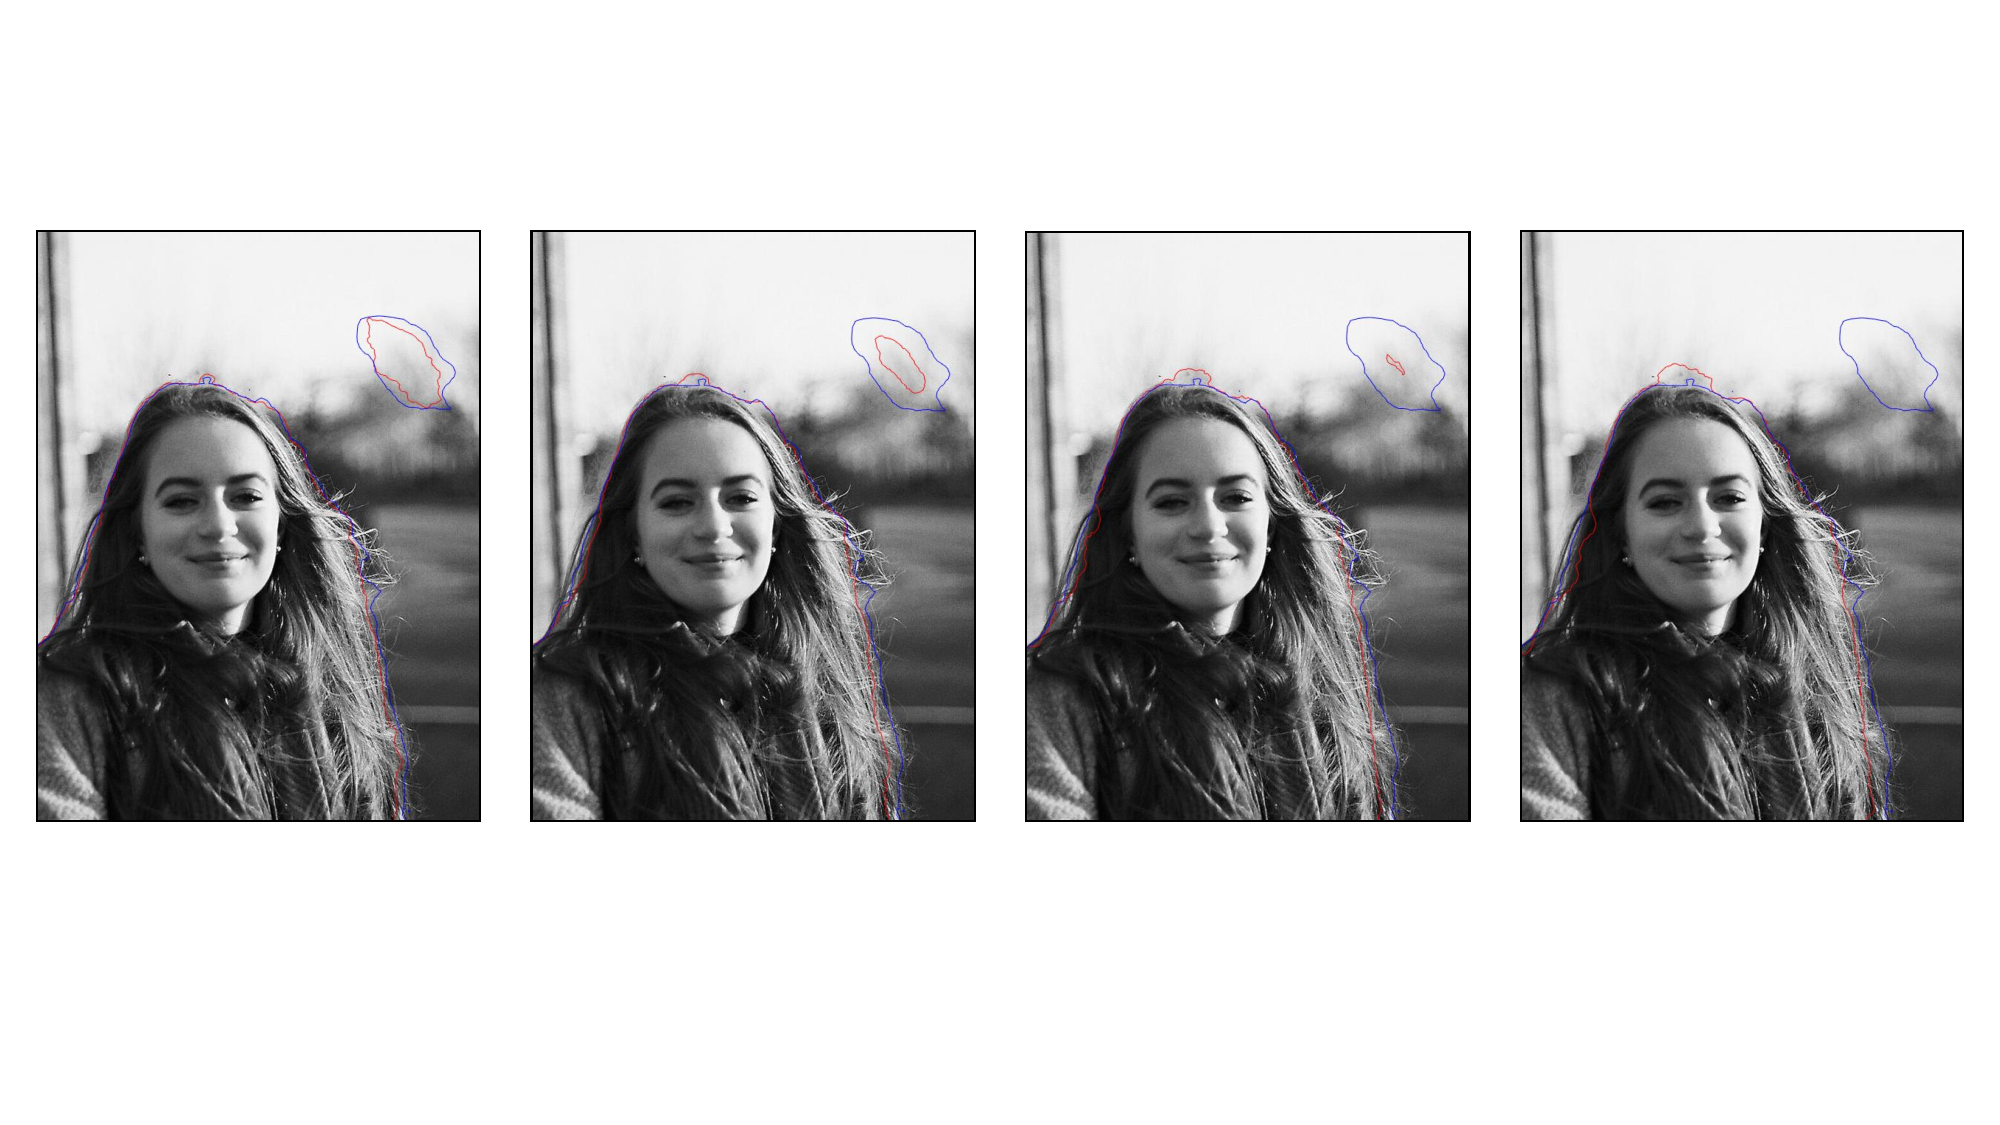
\includegraphics[width=8.8cm]{figs/Experiment1Result.eps}
    \caption{The contour evolution process of Experiment $1$.}
    \label{fig: The contour evolution process of Experiment 1}
\end{figure}
From the experiment result, it can be seen that the final segmentation result is more similar to the corrected prior shape. However, the corrected prior is imprecise, so the result of Experiment $1$ is inaccurate in the segmentation details.

\subsubsection{Experiment $2$}
There are some differences between experiment $1$ and experiment $2$. $\mathcal{E}_{\text{img}}$ only uses the original image information to capture the boundaries in the original picture.
\begin{equation}
\begin{split}
    \mathcal{E}_{\text{img}} & = \sum_{i=1}^2 \lambda_i \\
     &\cdot \int\left( \int K_\sigma(\mathbf{x}-\mathbf{y}) \left| I(\mathbf{y}) - f_i(\mathbf{x}) \right|^2 M_i(\phi(\mathbf{y}))\mathrm{d}\mathbf{y} \right)\mathrm{d}\mathbf{x}
\end{split}
\end{equation}
And the product of the probability map and the corrected prior shape can be obtained based on $Q_i(\mathbf{x}) = P_i(\mathbf{x})\cdot Smooth(S_i(\mathbf{x}))$ as shown in Fig. \ref{fig: The product of the probability map and the corrected prior shape}. $Smooth(S_i(\mathbf{x}))$ is the average smooth of the corrected prior shape.
\begin{figure}[h]
    \centering
    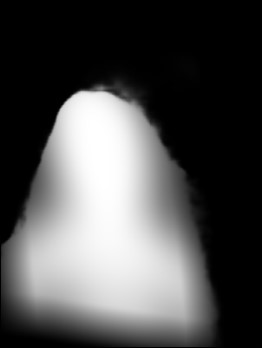
\includegraphics[width=2.7cm]{figs/Experiment2_plus.jpg}
    \caption{The product of the probability map and the corrected prior shape.}
    \label{fig: The product of the probability map and the corrected prior shape}
\end{figure}
Then, $\mathcal{E}_{\text{shape}}$ is redefined by Eq. (\ref{eq: Experiment 2 E_shape}).
\begin{equation}\label{eq: Experiment 2 E_shape}
    \mathcal{E}_{\text{shape}} = \sum_{i=1}^2 \pi_i \int Q_i(\mathbf{x}) M_i(\phi(\mathbf{x})) \mathrm{d}\mathbf{x}
\end{equation}
Experiment $2$ uses the intersection of the probability map and the corrected shape prior as the target shape regions. And then the boundary of target is located according to the information of the original image. The contour evolution process of Experiment $2$ is shown in Fig. \ref{fig: The contour evolution process of Experiment 2}.
\begin{figure}[h]
    \centering
    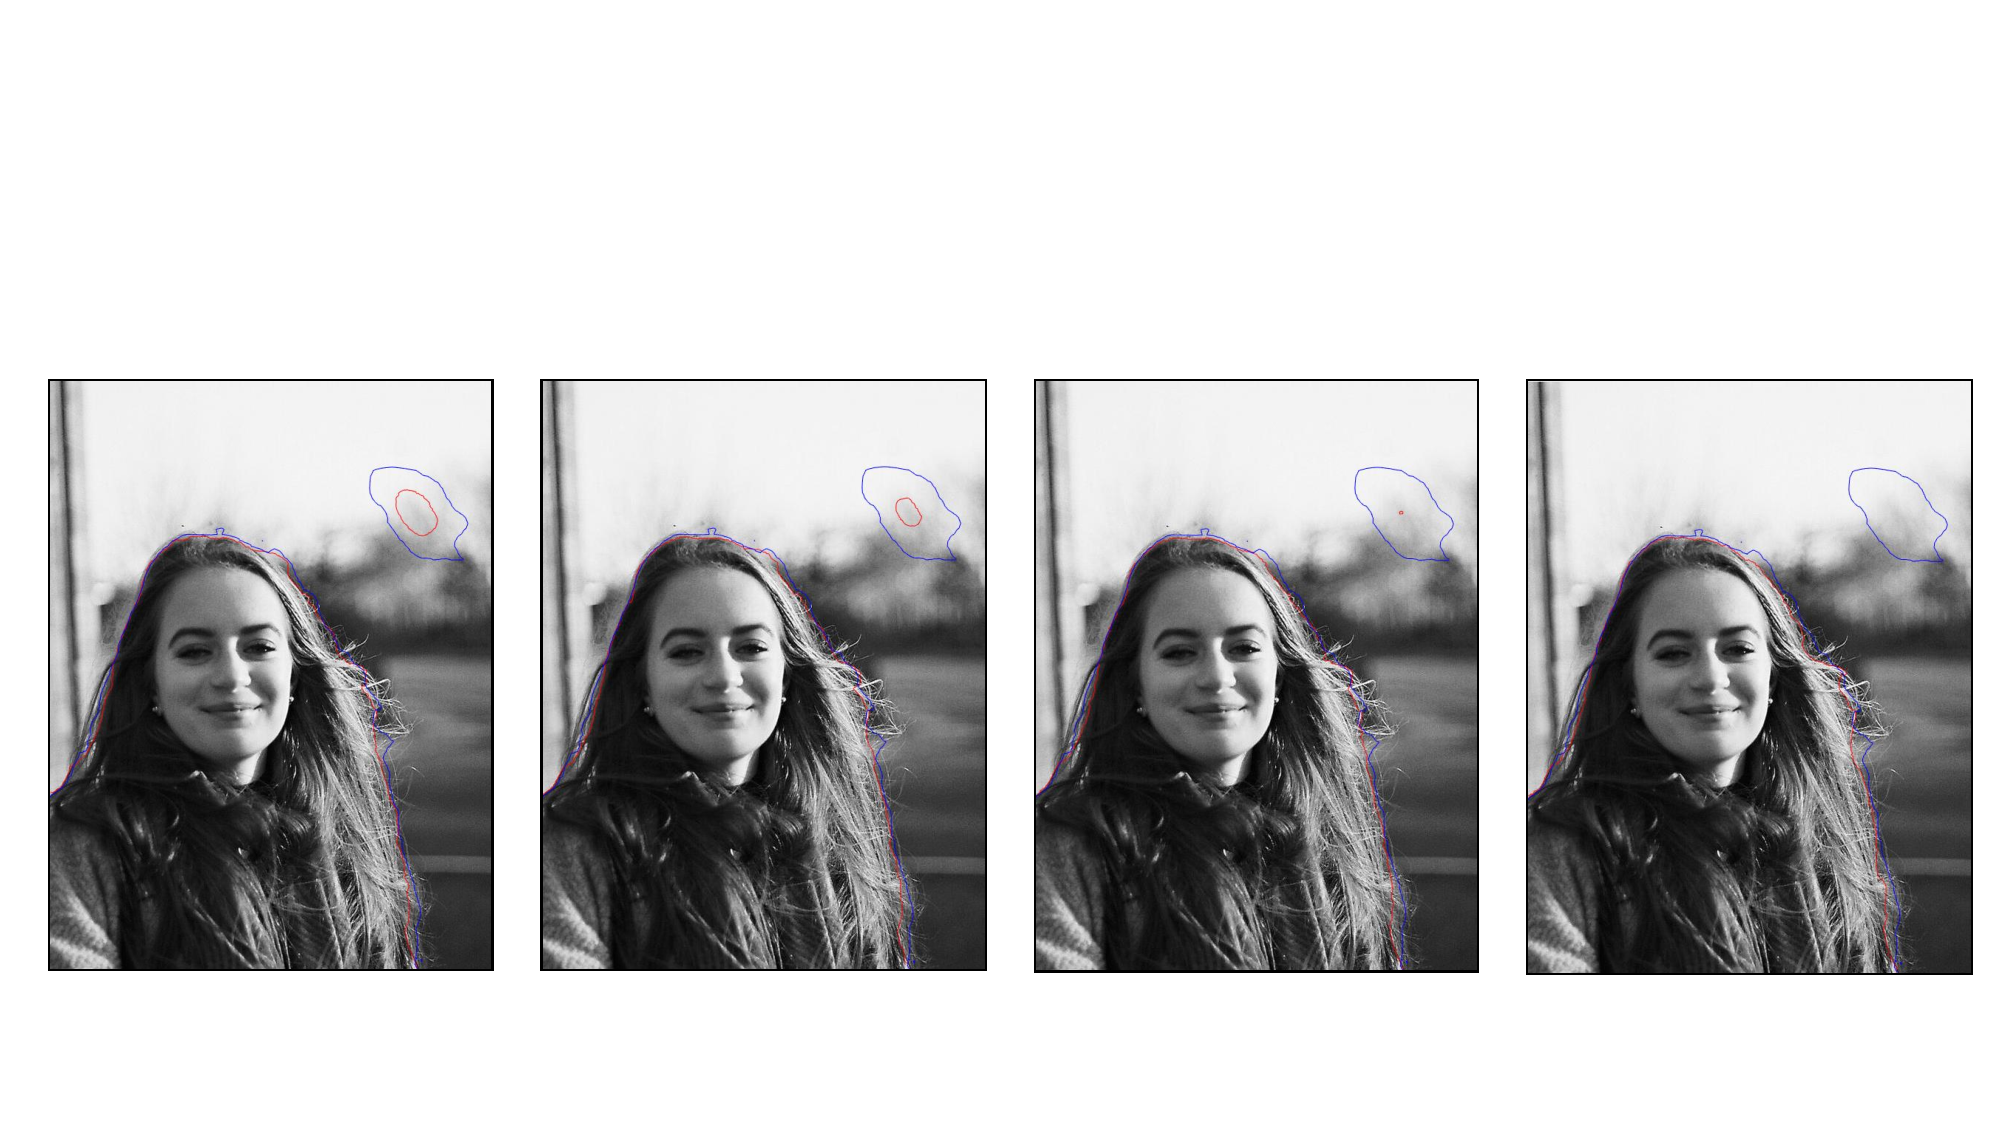
\includegraphics[width=8.8cm]{figs/Experiment2Result.eps}
    \caption{The contour evolution process of Experiment $2$.}
    \label{fig: The contour evolution process of Experiment 2}
\end{figure}
It can be seen from Fig. \ref{fig: The contour evolution process of Experiment 2} that the reference information method in Experiment $2$ can more accurately locate the boundary of the target.
